\documentclass[11pt,oneside]{article}
\usepackage[T1]{fontenc}
\usepackage[utf8]{inputenc}
% \usepackage{lmodern}
%\usepackage[adobe-utopia,uppercase=upright,greeklowercase=upright]{mathdesign}
\usepackage[adobe-utopia]{mathdesign}
%\usepackage{minionpro}
% \usepackage{pifont}
% \usepackage{amssymb}
\usepackage{amsmath}
\usepackage[francais]{babel}
% \usepackage[francais]{varioref}
\usepackage[dvips]{graphicx}

\usepackage{framed}
\usepackage[normalem]{ulem}
\usepackage{fancyhdr}
\usepackage{titlesec}
\usepackage{vmargin}
\usepackage{longtable}

\usepackage{ifthen}


%\usepackage{epsfig}
\usepackage{subfig}

\usepackage{multirow}
\usepackage{multicol} % Portions de texte en colonnes
\usepackage{flafter}%floatants après la référence



\usepackage{color}
\usepackage{colortbl}


\definecolor{gris25}{gray}{0.75}
\definecolor{bleu}{RGB}{18,33,98}
\definecolor{bleuf}{RGB}{42,94,171}
\definecolor{bleuc}{RGB}{231,239,247}
\definecolor{rougef}{RGB}{185,18,27}
\definecolor{rougec}{RGB}{255,230,231}
\definecolor{vertf}{RGB}{103,126,82}
\definecolor{vertc}{RGB}{220,255,191}
\definecolor{violetf}{RGB}{112,48,160}
\definecolor{violetc}{RGB}{230,224,236}

\newenvironment{sci}[1][\hsize]%
{%
    \def\FrameCommand%
    {%
%\rotatebox{90}{\textit{\textsf{Scilab}}
\includegraphics[height=.8cm]{png/logo_scilab}} 
\rotatebox{90}{
\includegraphics[height=.6cm]{png/logo_scilab}} 
        {\color{violetf}\vrule width 3pt}%
        \hspace{0pt}%must no space.
        \fboxsep=\FrameSep\colorbox{violetc}%
    }%
    \MakeFramed{\hsize #1 \advance\hsize-\width\FrameRestore}%
}%
{\endMakeFramed}%

\newenvironment{pseudo}[1][\hsize]%
{%
    \def\FrameCommand%
    {%
\rotatebox{90}{\textit{\textsf{Pseudo Code}}} 
        {\color{violetf}\vrule width 3pt}%
        \hspace{0pt}%must no space.
        \fboxsep=\FrameSep\colorbox{violetc}%
    }%
    \MakeFramed{\hsize #1 \advance\hsize-\width\FrameRestore}%
}%
{\endMakeFramed}%

\newenvironment{py}[1][\hsize]%
{%
    \def\FrameCommand%
    {%
%\rotatebox{90}{\textit{\textsf{Python}}} 
\rotatebox{90}{
\includegraphics[height=.6cm]{png/logo_python}} 
        {\color{violetf}\vrule width 3pt}%
        \hspace{0pt}%must no space.
        \fboxsep=\FrameSep\colorbox{violetc}%
    }%
    \MakeFramed{\hsize #1 \advance\hsize-\width\FrameRestore}%
}%
{\endMakeFramed}%


\newenvironment{corrige}[1][\hsize]%
{%
    \def\FrameCommand
    {%
\rotatebox{90}{\textit{\textsf{Correction}}} 
        {\color{violetf}\vrule width 3pt}%
        \hspace{0pt}%must no space.
        \fboxsep=\FrameSep\colorbox{violetc}%
    }%
    \MakeFramed{\hsize#1\advance\hsize-\width\FrameRestore}%
}%
{\endMakeFramed}%



\newenvironment{rem}[1][\hsize]%
{%
    \def\FrameCommand
    {%
\rotatebox{90}{\textit{\textsf{Remarque}}} 
        {\color{bleuf}\vrule width 3pt}%
        \hspace{0pt}%must no space.
        \fboxsep=\FrameSep\colorbox{bleuc}%
    }%
    \MakeFramed{\hsize#1\advance\hsize-\width\FrameRestore}%
}%
{\endMakeFramed}%


\newenvironment{savoir}[1][\hsize]%
{%
    \def\FrameCommand
    {%
\rotatebox{90}{\textit{\textsf{Savoir}}} 
        {\color{bleuf}\vrule width 3pt}%
        \hspace{0pt}%must no space.
        \fboxsep=\FrameSep\colorbox{bleuc}%
    }%
    \MakeFramed{\hsize#1\advance\hsize-\width\FrameRestore}%
}%
{\endMakeFramed}%

\newenvironment{prob}[1][\hsize]%
{%
    \def\FrameCommand%
    {%
\rotatebox{90}{\textit{\textsf{ Problématique}}} 
        {\color{rougef}\vrule width 3pt}%
        \hspace{0pt}%must no space.
        \fboxsep=\FrameSep\colorbox{rougec}%
    }%
    \MakeFramed{\hsize#1\advance\hsize-\width\FrameRestore}%
}%
{\endMakeFramed}%

\newenvironment{obj}[1][\hsize]%
{%
    \def\FrameCommand%
    {%
\rotatebox{90}{\textit{\textsf{Objectifs}}} 
        {\color{rougef}\vrule width 3pt}%
        \hspace{0pt}%must no space.
        \fboxsep=\FrameSep\colorbox{rougec}%
    }%
    \MakeFramed{\hsize#1\advance\hsize-\width\FrameRestore}%
}%
{\endMakeFramed}%

\newenvironment{defi}[1][\hsize]%
{%
    \def\FrameCommand%
    {%
\rotatebox{90}{\textit{\textsf{Définition\\}}} 
        {\color{bleuf}\vrule width 3pt}%
        \hspace{0pt}%must no space.
        \fboxsep=\FrameSep\colorbox{bleuc}%
    }%
    \MakeFramed{\hsize#1\advance\hsize-\width\FrameRestore}%
}%
{\endMakeFramed}%


\newenvironment{demo}[1][\hsize]%
{%
    \def\FrameCommand%
    {%
\rotatebox{90}{\textit{\textsf{Démonstration\\}}} 
        {\color{bleuf}\vrule width 3pt}%
        \hspace{0pt}%must no space.
        \fboxsep=\FrameSep\colorbox{bleuc}%
    }%
    \MakeFramed{\hsize#1\advance\hsize-\width\FrameRestore}%
}%
{\endMakeFramed}%


\newenvironment{hypo}[1][\hsize]%
{%
    \def\FrameCommand%
    {%
\rotatebox{90}{\textit{\textsf{Hypothèse\\}}} 
        {\color{bleuf}\vrule width 3pt}%
        \hspace{0pt}%must no space.
        \fboxsep=\FrameSep\colorbox{bleuc}%
    }%
    \MakeFramed{\hsize#1\advance\hsize-\width\FrameRestore}%
}%
{\endMakeFramed}%


\newenvironment{prop}[1][\hsize]%
{%
    \def\FrameCommand%
    {%
\rotatebox{90}{\textit{\textsf{Propriété\\}}} 
        {\color{bleuf}\vrule width 3pt}%
        \hspace{0pt}%must no space.
        \fboxsep=\FrameSep\colorbox{bleuc}%
    }%
    \MakeFramed{\hsize#1\advance\hsize-\width\FrameRestore}%
}%
{\endMakeFramed}%

\newenvironment{props}[1][\hsize]%
{%
    \def\FrameCommand%
    {%
\rotatebox{90}{\textit{\textsf{Propriétés\\}}} 
        {\color{bleuf}\vrule width 3pt}%
        \hspace{0pt}%must no space.
        \fboxsep=\FrameSep\colorbox{bleuc}%
    }%
    \MakeFramed{\hsize#1\advance\hsize-\width\FrameRestore}%
}%
{\endMakeFramed}%

\newenvironment{exemple}[1][\hsize]%
{%
    \def\FrameCommand%
    {%
\rotatebox{90}{\textit{\textsf{Exemple\\}}} 
        {\color{vertf}\vrule width 3pt}%
        \hspace{0pt}%must no space.
        \fboxsep=\FrameSep\colorbox{vertc}%
    }%
    \MakeFramed{\hsize#1\advance\hsize-\width\FrameRestore}%
}%
{\endMakeFramed}%

\newenvironment{resultat}[1][\hsize]%
{%
    \def\FrameCommand%
    {%
\rotatebox{90}{\textit{\textsf{Résultat\\}}} 
        {\color{rougef}\vrule width 3pt}%
        \hspace{0pt}%must no space.
        \fboxsep=\FrameSep\colorbox{rougec}%
    }%
    \MakeFramed{\hsize#1\advance\hsize-\width\FrameRestore}%
}%
{\endMakeFramed}%

\newenvironment{methode}[1][\hsize]%
{%
    \def\FrameCommand%
    {%
\rotatebox{90}{\textit{\textsf{Méthode\\}}} 
        {\color{rougef}\vrule width 3pt}%
        \hspace{0pt}%must no space.
        \fboxsep=\FrameSep\colorbox{rougec}%
    }%
    \MakeFramed{\hsize#1\advance\hsize-\width\FrameRestore}%
}%
{\endMakeFramed}%

\newenvironment{theo}[1][\hsize]%
{%
    \def\FrameCommand%
    {%
\rotatebox{90}{\textit{\textsf{Théorème\\}}} 
        {\color{rougef}\vrule width 3pt}%
        \hspace{0pt}%must no space.
        \fboxsep=\FrameSep\colorbox{rougec}%
    }%
    \MakeFramed{\hsize#1\advance\hsize-\width\FrameRestore}%
}%
{\endMakeFramed}%

\newenvironment{warn}[1][\hsize]%
{%
    \def\FrameCommand%
    {%
\rotatebox{90}{\textit{\textsf{Attention\\}}} 
        {\color{rougef}\vrule width 3pt}%
        \hspace{0pt}%must no space.
        \fboxsep=\FrameSep\colorbox{rougec}%
    }%
    \MakeFramed{\hsize#1\advance\hsize-\width\FrameRestore}%
}%
{\endMakeFramed}%

% \usepackage{pstricks}
%\usepackage{minitoc}
% \setcounter{minitocdepth}{4}

\setcounter{tocdepth}{2}

% \mtcselectlanguage{french} 

%\usepackage{draftcopy}% "Brouillon"
% \usepackage{floatflt}
\usepackage{psfrag}
%\usepackage{listings} % Permet d'insérer du code de programmation
\renewcommand{\baselinestretch}{1.2}

% Changer la numérotation des figures :
% ------------------------------------
% \makeatletter
% \renewcommand{\thefigure}{\ifnum \c@section>\z@ \thesection.\fi
%  \@arabic\c@figure}
% \@addtoreset{figure}{section}
% \makeatother
 


%%%%%%%%%%%%
% Définition des vecteurs %
%%%%%%%%%%%%
 \newcommand{\vect}[1]{\overrightarrow{#1}}

%%%%%%%%%%%%
% Définition des torseusr %
%%%%%%%%%%%%

 \newcommand{\torseur}[1]{%
\left\{{#1}\right\}
}

\newcommand{\torseurcin}[3]{%
\left\{\mathcal{#1} \left(#2/#3 \right) \right\}
}

\newcommand{\torseurstat}[3]{%
\left\{\mathcal{#1} \left(#2\rightarrow #3 \right) \right\}
}

 \newcommand{\torseurc}[8]{%
%\left\{#1 \right\}=
\left\{
{#1}
\right\}
 = 
\left\{%
\begin{array}{cc}%
{#2} & {#5}\\%
{#3} & {#6}\\%
{#4} & {#7}\\%
\end{array}%
\right\}_{#8}%
}

 \newcommand{\torseurcol}[7]{
\left\{%
\begin{array}{cc}%
{#1} & {#4}\\%
{#2} & {#5}\\%
{#3} & {#6}\\%
\end{array}%
\right\}_{#7}%
}

 \newcommand{\torseurl}[3]{%
%\left\{\mathcal{#1}\right\}_{#2}=%
\left\{%
\begin{array}{l}%
{#1} \\%
{#2} %
\end{array}%
\right\}_{#3}%
}

 \newcommand{\vectv}[3]{%
\vect{V\left( {#1} \in {#2}/{#3}\right)}
}


\newcommand{\vectf}[2]{%
\vect{R\left( {#1} \rightarrow {#2}\right)}
}

\newcommand{\vectm}[3]{%
\vect{\mathcal{M}\left( {#1}, {#2} \rightarrow {#3}\right)}
}


 \newcommand{\vectg}[3]{%
\vect{\Gamma \left( {#1} \in {#2}/{#3}\right)}
}

 \newcommand{\vecto}[2]{%
\vect{\Omega\left( {#1}/{#2}\right)}
}
% }$$\left\{\mathcal{#1} \right\}_{#2} =%
% \left\{%
% \begin{array}{c}%
%  #3 \\%
%  #4 %
% \end{array}%
% \right\}_{#5}}

%  ------------------------------------------
% | Modification du formatage des sections : | 
%  ------------------------------------------

% Grands titres :
% ---------------

\newcommand{\titre}[1]{%
\begin{center}
      \bigskip
      \rule{\textwidth}{1pt}
      \par\vspace{0.1cm}
      
      \textbf{\large #1}
      \par\rule{\textwidth}{1pt}
    \end{center}
    \bigskip
  }

% Supprime le numéro du chapitre dans la numérotation des sections:
% -----------------------------------------------------------------
\makeatletter
\renewcommand{\thesection}{\@arabic\c@section}
\makeatother


% \titleformat{\chapter}[display]
% {\normalfont\Large\filcenter}
% {}
% {1pc}
% {\titlerule[1pt]
%   \vspace{1pc}%
%   \Huge}[\vspace{1ex}%
% \titlerule]


%%%% Chapitres Comme PY Pechard %%%%%%%%%
% numéro du chapitre
\DeclareFixedFont{\chapnumfont}{OT1}{phv}{b}{n}{80pt}
% pour le mot « Chapitre »
\DeclareFixedFont{\chapchapfont}{OT1}{phv}{m}{it}{40pt}
% pour le titre
\DeclareFixedFont{\chaptitfont}{T1}{phv}{b}{n}{25pt}

\definecolor{gris}{gray}{0.75}
\titleformat{\chapter}[display]%
	{\sffamily}%
	{\filleft\chapchapfont\color{gris}\chaptertitlename\
	\\
	\vspace{12pt}
	\chapnumfont\thechapter}%
	{16pt}%
	{\filleft\chaptitfont}%
	[\vspace{6pt}\titlerule\titlerule\titlerule]

%%%%  Fin Chapitres Comme PY Pechard %%%%%%%%%


% Section, subsection, subsubsection sans serifs :
% % ----------------------------------------------

% \makeatletter
% \renewcommand{\section}{\@startsection{section}{0}{0mm}%
% {\baselineskip}{.3\baselineskip}%
% {\normalfont\sffamily\Large\textbf}}%
% \makeatother

\makeatletter
\renewcommand{\@seccntformat}[1]{{\textcolor{bleu}{\csname
the#1\endcsname}\hspace{0.5em}}}
\makeatother

\makeatletter
\renewcommand{\section}{\@startsection{section}{1}{\z@}%
                       {-4ex \@plus -1ex \@minus -.4ex}%
                       {1ex \@plus.2ex }%
                       {\normalfont\Large\sffamily\bfseries}}%
\makeatother
 
\makeatletter
\renewcommand{\subsection}{\@startsection {subsection}{2}{\z@}
                          {-3ex \@plus -0.1ex \@minus -.4ex}%
                          {0.5ex \@plus.2ex }%
                          {\normalfont\large\sffamily\bfseries}}
\makeatother
 
\makeatletter
\renewcommand{\subsubsection}{\@startsection {subsubsection}{3}{\z@}
                          {-2ex \@plus -0.1ex \@minus -.2ex}%
                          {0.2ex \@plus.2ex }%
                          {\normalfont\large\sffamily\bfseries}}
\makeatother
 
\makeatletter             
\renewcommand{\paragraph}{\@startsection{paragraph}{4}{\z@}%
                                    {-2ex \@plus-.2ex \@minus .2ex}%
                                    {0.1ex}%               
{\normalfont\sffamily\bfseries}}
\makeatother
 

\makeatletter             
\renewcommand{\subparagraph}{\@startsection{subparagraph}{5}{\z@}%
                                    {-2ex \@plus-.2ex \@minus .2ex}%
                                    {0.1ex}%               
{\normalfont\bfseries Question }}
\makeatother

\renewcommand{\thesubparagraph}{\arabic{subparagraph}} 
\makeatletter

\setcounter{secnumdepth}{5}
%\renewcommand{\subparagraph}{\@startsection{subparagraph}{5}{\z@}%
%                                       {-2ex \@plus-.1ex \@minus .2ex}%
%                                       {0.1ex}%
%				    {\normalfont\normalsize\sffamily\bfseries}}
%\makeatletter
% \makeatletter
% \renewcommand{\subsection}{\@startsection{subsection}{1}{2mm}%
% {\baselineskip}{.3\baselineskip}%
% {\normalfont\sffamily\large\textbf}}%
% \makeatother
% 
% \makeatletter
% \renewcommand{\subsubsection}{\@startsection{subsubsection}{2}{4mm}%
% {\baselineskip}{.15\baselineskip}%
% {\normalfont\sffamily\large\textbf}}%
% \makeatother
% 
% \makeatletter
% \renewcommand{\paragraph}{\@startsection{paragraph}{3}{6mm}%
% {\baselineskip}{.15\baselineskip}%
% {\normalfont\sffamily\large\textbf}}%
% \makeatother
 



%  --------
% | Marges |
%  --------


% \setmarginsrb{2.5cm}{1.5cm}{2.5cm}{2cm}{1cm}{1cm}{1cm}{1cm}
\setmarginsrb{1.5cm}{1cm}{1cm}{1.5cm}{1cm}{1cm}{1cm}{1cm}

% Changer les marges localement :
% -----------------------------
\newenvironment{changemargin}[2]{\begin{list}{}{%
\setlength{\topsep}{0pt}%
\setlength{\leftmargin}{0pt}%
\setlength{\rightmargin}{0pt}%
\setlength{\listparindent}{\parindent}%
\setlength{\itemindent}{\parindent}%
\setlength{\parsep}{0pt plus 1pt}%
\addtolength{\leftmargin}{#1}%
\addtolength{\rightmargin}{#2}%
}\item }{\end{list}}



\usepackage{pst-solides3d}
\usepackage{titletoc}
\titlecontents{chapter}[+3pc]
  {\addvspace{10pt}\sffamily\bfseries}
{\contentslabel[{\pscirclebox[fillstyle=solid,fillcolor=gray!25,
linecolor=gray!25,framesep=4pt]{\textcolor{white}{\thecontentslabel}}}]{2.5pc}}
  {}
  {\dotfill \normalfont\thecontentspage\ }

\titlecontents{section}[3pc]
  {\addvspace{2pt}\sffamily}
  {\contentslabel[\thecontentslabel]{1.8pc}}
  {}
  {\dotfill \normalfont\thecontentspage\ }

\titlecontents{subsection}[5pc]
  {\addvspace{2pt}\sffamily}
  {\contentslabel[\thecontentslabel]{1.8pc}}
  {}
  {\dotfill \normalfont\thecontentspage\ }

\titlecontents{subsubsection}[8pc]
  {\addvspace{2pt}\sffamily}
  {\contentslabel[\thecontentslabel]{3pc}}
  {}
  {\dotfill \normalfont\thecontentspage\ }
%{\;\titlerule\;\normalfont\thecontentspage\ }

\titlecontents{paragraph}[9pc]
  {\addvspace{2pt}\sffamily}
  {\contentslabel[\thecontentslabel]{3.5pc}}
  {}
  {\dotfill \normalfont\thecontentspage\ }




\usepackage{style/schemabloc}
%Si le boolen xp est vrai : compilation pour xabi
%Sinon compilation Damien
\newboolean{xp}
\setboolean{xp}{true}

\newboolean{prof}
\setboolean{prof}{false}

\def\xxtitre{\ifthenelse{\boolean{xp}}{
CI 2 -- SLCI : Étude du comportement des Systèmes Linéaires Continus Invariants}{
}}

\def\xxsoustitre{\ifthenelse{\boolean{xp}}{
Devoir Maison 4}{
}}


\def\xxauteur{\ifthenelse{\boolean{xp}}{
\noindent 2013 -- 2014 \\
Xavier \textsc{Pessoles}}{
}}


\def\xxpied{\ifthenelse{\boolean{xp}}{
CI 2 : SLCI\\
DM 4 : \ifthenelse{\boolean{prof}}{P}{E}%
}{
}}

\usepackage[%
    pdftitle={SLCI - Systèmes du second ordre},
    pdfauthor={Xavier Pessoles},
    colorlinks=true,
    linkcolor=blue,
    citecolor=magenta]{hyperref}



\usepackage{pifont}
\sloppy
\hyphenpenalty 10000


\begin{document}






% \makeatletter \let\ps@plain\ps@empty \makeatother
%% DEBUT DU DOCUMENT
%% =================




%------------- En tetes et Pieds de Pages ------------


\pagestyle{fancy}
\ifthenelse{\boolean{xp}}{%
\renewcommand{\headrulewidth}{0pt}}{%
\renewcommand{\headrulewidth}{0.2pt}} %pour mettre le trait en haut
%\renewcommand{\headrulewidth}{0.2pt}

\fancyhead{}
\fancyhead[L]{%
\ifthenelse{\boolean{xp}}{%
\noindent\begin{minipage}[c]{2.6cm}%

\includegraphics[width=2cm]{png/logo_ptsi.png}%
\end{minipage}%
}{%
\footnotesize{\textit{\textsf{Lycée François Premier}}}
}}

\ifthenelse{\boolean{xp}}{%
\fancyhead[C]{\rule{12cm}{.5pt}}}{
}


\fancyhead[R]{%
\noindent\begin{minipage}[c]{3cm}
\begin{flushright}
\footnotesize{\textit{\textsf{Sciences Industrielles \\ de l'ingénieur}}}%
\end{flushright}
\end{minipage}
}


\ifthenelse{\boolean{xp}}{%
\fancyhead[C]{\rule{12cm}{.5pt}}}{
}

\renewcommand{\footrulewidth}{0.2pt}

\fancyfoot[C]{\footnotesize{\bfseries \thepage}}
\fancyfoot[L]{%
\begin{minipage}[c]{.2\linewidth}
\noindent\footnotesize{{\xxauteur}}
\end{minipage}
\ifthenelse{\boolean{xp}}{}{%
\begin{minipage}[c]{.15\linewidth}

\includegraphics[width=2cm]{png/logoCC.png}
\end{minipage}}
}


\fancyfoot[R]{\footnotesize{\xxpied}}



\begin{center}
 \Large\textsc{\xxtitre}
\end{center}

\begin{center}
 \large\textsc{\xxsoustitre}
\end{center}

%\vspace{.5cm}

\begin{center}
 \large\textsc{Robot préhenseur}
\end{center}

\ifthenelse{\boolean{prof}}{\begin{flushright}
\textit{D'après ressources Florestan Mathurin.}
\end{flushright}}{}




\ifthenelse{\boolean{prof}}{}{
\begin{minipage}[c]{.3\linewidth}
\begin{center}
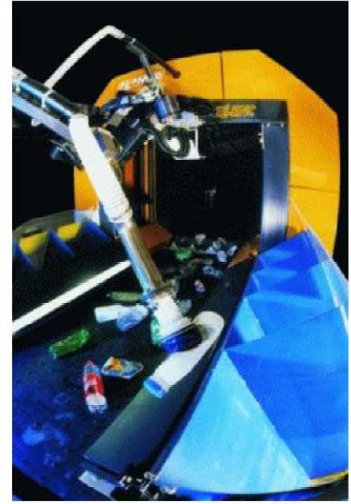
\includegraphics[width=.95\textwidth]{png/fig2_2}
\end{center}
\end{minipage}\hfill
\begin{minipage}[c]{.65\linewidth}
Le support de l'étude est un préhenseur de pièces. Il permet à l'utilisateur de prendre des pièces pour les déplacer. L'application illustrée sur l'image ci-dessous est la prise de bouteilles plastiques sur un tapis roulant, afin de les trier pour faire du recyclage. 

Le système doit répondre aux exigences suivantes : 
\begin{itemize}
\item Req 1 : Permettre à l'utilisateur de prendre des pièces;
\item Req 2 : S'adapter au bâti;
\item Req 3 : S'adapter à l'énergie;
\item Req 4 : Respecter les normes industrielles.
\end{itemize}

\begin{center}
\begin{tabular}{|l|l|l|}
\hline
Fonction & Critère & Niveau \\
\hline
Req 1  & Rapidité & $t_{5\%}\leq 0,2 \; s.$ \\
\hline
\end{tabular}
\end{center}
\end{minipage}
\vspace{0.25cm}
%\begin{minipage}[c]{.3\linewidth}
%\begin{center}
%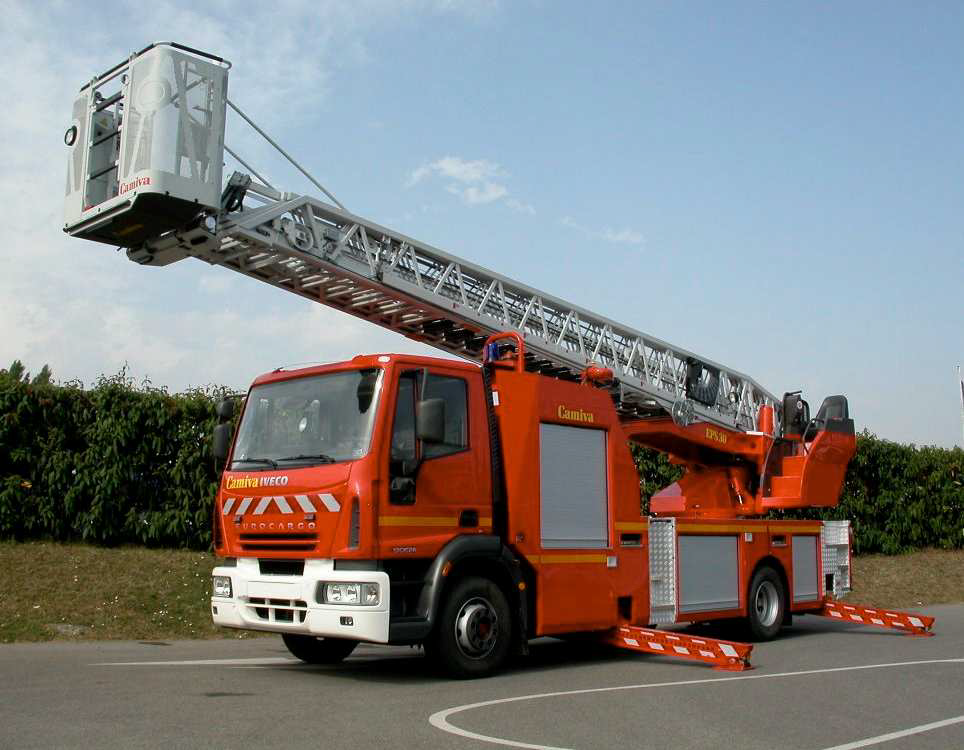
\includegraphics[width=.9\textwidth]{png/fig1}
%\end{center}
%\end{minipage}\hfill
%\begin{minipage}[c]{.65\linewidth}
%\begin{center}
%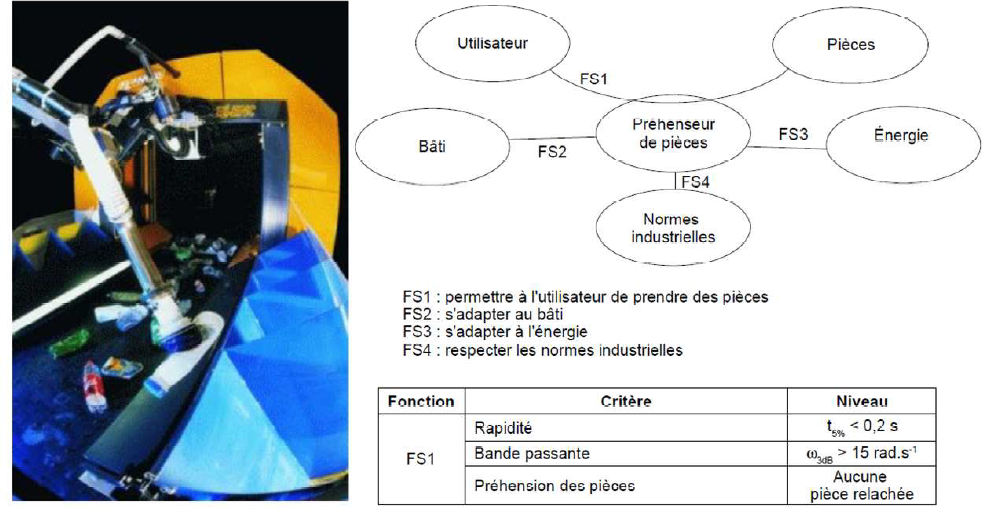
\includegraphics[width=.9\textwidth]{png/fig2}
%\end{center}
%\end{minipage}

L'objectif de cette étude est de vérifier que l'exigence Req 1 est respectée. On réalise l'asservissement de la position angulaire d'un bras du préhenseur de pièces, selon le schéma bloc qui suit (l'angle du bras $\theta_b(t)$, l'angle consigne est $\theta_c(t)$).

\begin{center}
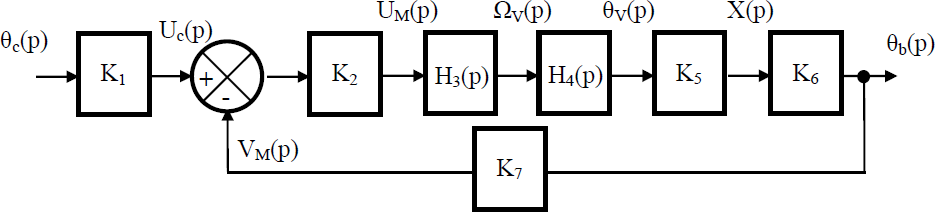
\includegraphics[width=.9\textwidth]{png/fig_3}
\end{center}

Avec $K_1$, $K_2$, $K_5$, $K_6$ et $K_7$ : constantes, $\theta_c(p)$ : angle de consigne, $U_c(p)$ : tension de consigne, $U_M(p)$, tension moteur, $\Omega_V(p)$ : vitesse angulaire de la vis, $\theta_V(p)$ : angle de la vis, $X(p)$ : déplacement de l'écrou, $\dot{\theta_b(p)}$ : position angulaire du bras, $V_M(p)$ : tension mesurée image de $\theta_b(p)$.
}

\subparagraph{}
\textit{Déterminer le lien entre $K_1$ et $K_7$ pour que $\theta_b(p)$ soit asservi sur $\theta_c(p)$.}
\ifthenelse{\boolean{prof}}{
\begin{corrige}
Les blocs $K_1$ et $K_7$ servent tous les deux à convertir une position angulaire en tension. De plus, ces tensions étant soustraites par le comparateur, il faut qu'elles aient le même ordre de grandeur. 

Enfin, dans l'hypothèse le système est précis, on a nécessairement, en régime permanent,  $\theta_c(t) = \theta_b(t)$, et $U_c(t)-V_M(t)=0$. En conclusion on a nécessairement $K_1 = K_7$.
\end{corrige}
}{}

\ifthenelse{\boolean{prof}}{}{
La fonction de transfert $H_3(p)$ est réalisée par un moteur, dont les équations de comportement sont :
$$
u_M(t)=e(t)+R\cdot i(t) \quad e(t)=k_e\omega_v(t) \quad J\cdot \dfrac{d\omega_v(t)}{dt}=C_M(t) \quad C_M(t)=k_M i(t)
$$

Avec $u_M(t)$ : tension aux bornes du moteur (en V), $e(t)$ : force contre-électromotrice (en V), $i(t)$ intensité (en A), $\omega_V(t)$ : vitesse de rotation de la vis en sortie de moteur (en rad/s), $C_M(t)$ ; couple moteur (en N.m) (un couple est une action mécanique qui tend à faire tourner). $J$ inertie équivalente en rotation de l'arbre moteur (en $kg\cdot m^2$), $R$ résistance du moteur (en $\Omega$), $k_e$ constante de force contre-électrmotrice ($V\cdot rad^{-1}\cdot s$), $k_m$ : constante de couple ($N\cdot m\cdot A^{-1}$).
}

\subparagraph{}
\textit{Déterminer la fonction de transfert $H_3(p)=\dfrac{\Omega_V(p)}{U_M(p)}$. Montrer que $H_3(p)$ peut se mettre sous la forme canonique d'un système du premier ordre où les valeurs $K_3$ et $T_3$ seront à déterminer.}

\ifthenelse{\boolean{prof}}{
\begin{corrige}
En utilisant les équations, on a : 
$$
U_M(p)=E(p)+R\cdot I(p) 
\Longleftrightarrow U_M(p)=k_e\Omega_v(p)+R \cdot \dfrac{C_M(p)}{k_m}
\Longleftrightarrow U_M(p)=k_e\Omega_v(p)+R \cdot \dfrac{J}{k_m} \cdot p \Omega_v(p)
$$

En conséquences, 
$$
U_M(p)= \Omega_v(p)\left( k_e+R \cdot \dfrac{Jp}{k_m} \right)
$$
 et donc, 

$$
H_3(p)=\dfrac{\Omega_v(p)}{U_M(p)} 
= \dfrac{1}{k_e+R \cdot \dfrac{Jp}{k_m}}
= \dfrac{1/k_e}{1+ \dfrac{RJ}{k_m k_e}p}
$$
\end{corrige}
}{}


\subparagraph{}
\textit{Déterminer $\omega_v(t)$ lorsque $u_M(t)$ est un échelon de tension d'amplitude $U_0$. Préciser la valeur de $\omega_v(t)$ à l'origine, la pente de la tangente à l'origine de $\omega_V(t)$ et la valeur finale atteinte par $\omega_V(t)$ lorsque $t$ tend vers l'infini.}
\ifthenelse{\boolean{prof}}{
\begin{corrige}
La fonction de transfert ayant été mis sous forme canonique à la question précédente, on peut directement donner la réponse du système à un échelon :
$$
\omega_v(t)=\dfrac{U_0}{k_e}\cdot\left(1-e^{-\dfrac{t}{\dfrac{RJ}{k_m k_e}}}\right)
$$

La valeur initiale est 0, la valeur finale vaut $\dfrac{U_0}{k_e}$, la pente à l'origine vaut $\dfrac{U_0}{k_e}\cdot \dfrac{k_m k_e}{RJ}$.
\end{corrige}
}{}


\subparagraph{}
\textit{Déterminer la fonction de transfert $H_4(p)$. }
\ifthenelse{\boolean{prof}}{
\begin{corrige}
On a $\dfrac{d\theta_V(t)}{dt} = \omega_V(t)$. En conséquences, $\dfrac{\Theta_V(p)}{\Omega_V(p)}=\dfrac{1}{p}$.
\end{corrige}
}{}


\subparagraph{}
\textit{Déterminer la fonction de transfert $H(p)=\dfrac{\theta_b(p)}{\theta_c(p)}$. Montrer que cette fonction peut se mettre sous la forme d'un système du second ordre ou les valeurs de $K$, $z$ et $\omega_0$ seront à déterminer.}
\ifthenelse{\boolean{prof}}{
\begin{corrige}
On a: 
$$
H(p)
=K_1 \cdot \dfrac{K_2\cdot H_3(p)\cdot H_4(p)\cdot K_5\cdot K_6}{1+K_2\cdot H_3(p)\cdot H_4(p)\cdot K_5\cdot K_6} 
=K_1 \cdot \dfrac{K_2\cdot \dfrac {K_m}{1+\tau_M p}\cdot \dfrac{1}{p}\cdot K_5\cdot K_6}{1+K_2\cdot  \dfrac{K_m}{1+\tau_M p}\cdot \dfrac{1}{p} \cdot K_5\cdot K_6 \cdot K_1} 
$$
$$
H(p)
=K_1 \cdot \dfrac{K_2\cdot K_m\cdot K_5\cdot K_6}{\left(1+\tau_M p\right)p+K_2\cdot  K_m  \cdot K_5\cdot K_6 \cdot K_1} 
$$

$$
H(p)
= \dfrac{\dfrac{K_1 K_2 K_m K_5  K_6}{K_2 K_m  K_5 K_6  K_1}}{\dfrac{1}{K_2 K_m  K_5 K_6  K_1}p+\dfrac{\tau_M}{K_2 K_m  K_5 K_6  K_1} p^2 +1} 
= \dfrac{1}{\dfrac{1}{K_2 K_m  K_5 K_6  K_1}p+\dfrac{\tau_M}{K_2 K_m  K_5 K_6  K_1} p^2 +1} 
$$

On a donc : 
\begin{itemize}
\item $K=1$;
\item $\dfrac{1}{\omega_0^2}=\dfrac{\tau_M}{K_2 K_m  K_5 K_6  K_1} \Longleftrightarrow \omega_0 = \sqrt{\dfrac{K_2 K_m  K_5 K_6  K_1}{\tau_M}}$;
\item $\dfrac{2 z}{\omega_0}=\dfrac{1}{K_2 K_m  K_5 K_6  K_1} \Longleftrightarrow
z =\dfrac{\omega_0}{2K_2 K_m  K_5 K_6  K_1} 
= \dfrac{\sqrt{\dfrac{K_2 K_m  K_5 K_6  K_1}{\tau_M}}}{2K_2 K_m  K_5 K_6  K_1}
= \dfrac{1}{2\sqrt{K_2 K_m  K_5 K_6  K_1\tau_M}}$.
\end{itemize}

\end{corrige}
}{}

\ifthenelse{\boolean{prof}}{}{
La réponse indicielle de $H(p)$ à un échelon unitaire est donnée sur la figure suivante :

\begin{center}
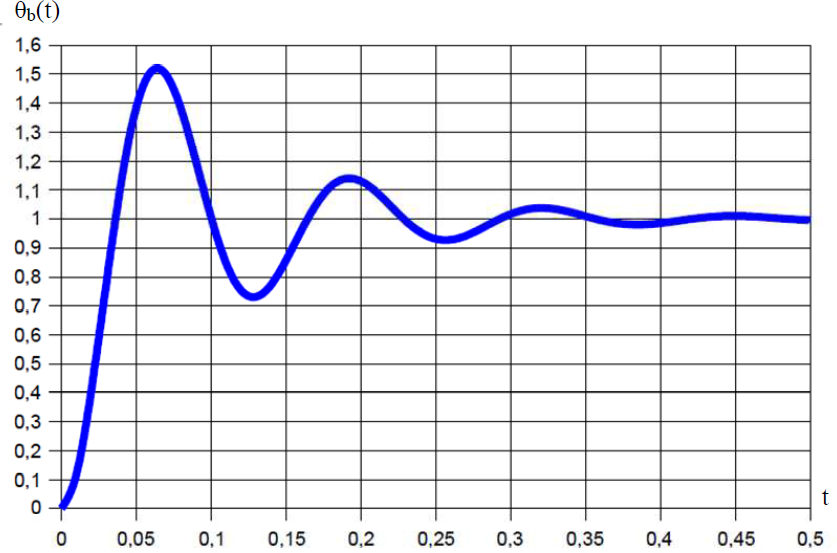
\includegraphics[width=.9\textwidth]{png/fig_4}
\end{center}
}
\subparagraph{}
\textit{Déterminer, en expliquant la méthode, les valeurs numériques de $K$, $z$ et $\omega_0$.}
\ifthenelse{\boolean{prof}}{
\begin{corrige}
Pour une entrée indicielle, $\theta_c(t)=1$ pour $t>0$. Or, $\theta_c(t)$ tend vers 1, on a donc $K=1$. 

Le premier dépassement a une valeur de 50\%.

Or, 
$$
D_{1\%}=0,5 = e^{\dfrac{-\pi \xi}{\sqrt{1-\xi^2}}} 
\Longrightarrow
\ln(0,5) = \dfrac{-\pi \xi}{\sqrt{1-\xi^2}}
\Longrightarrow
\ln(0,5) \sqrt{1-\xi^2} = -\pi \xi
\Longrightarrow
(\ln(0,5))^2 \left(1-\xi^2\right) - \pi^2 \xi^2 = 0
$$

$$
\Longrightarrow 
1-\xi^2 -\dfrac{\pi^2 \xi^2}{(\ln(0,5))^2} = 0
\Longrightarrow 
\xi^2 = \dfrac{1}{\dfrac{\pi^2}{(\ln(0,5))^2}+1}
\Longrightarrow 
\xi = \dfrac{(\ln(0,5))^2}{\pi^2+(\ln(0,5))^2}
\simeq 0,47
$$

Enfin, la pseudo période est d'environ 0,125 seconde. On a donc : 
$$
0,125 = \dfrac{2\pi}{\omega_0\sqrt{1-\xi^2}} 
\Longleftrightarrow 
\omega_0 = \dfrac{2\pi}{0,125 \sqrt{1-\xi^2}}  \simeq 57\; s^{-1}
$$

\end{corrige}
}{}


\subparagraph{}
\textit{Déterminer, en expliquant la démarche utilisée, le temps de réponse à 5\%. Conclure quant à la capacité du préhenseur à vérifier (ou non) le critère de rapidité de Req 1.}
\ifthenelse{\boolean{prof}}{
\begin{corrige}
En traçant la bande à plus et moins 5\% de la valeur finale, on constate que la courbe n'en sort plus à partir de $t=0,325\; s.$. En conséquences, l'exigence Req 1 n'est pas respectée. 

\end{corrige}
}{}


\end{document}
